I am studying the heterogeneity on education using the categories - High school dropout, High school graduate, Some college, College completed (4+ years), Post graduate.

\subsection*{Part 1}

\begin{figure}[H]
  \centering
  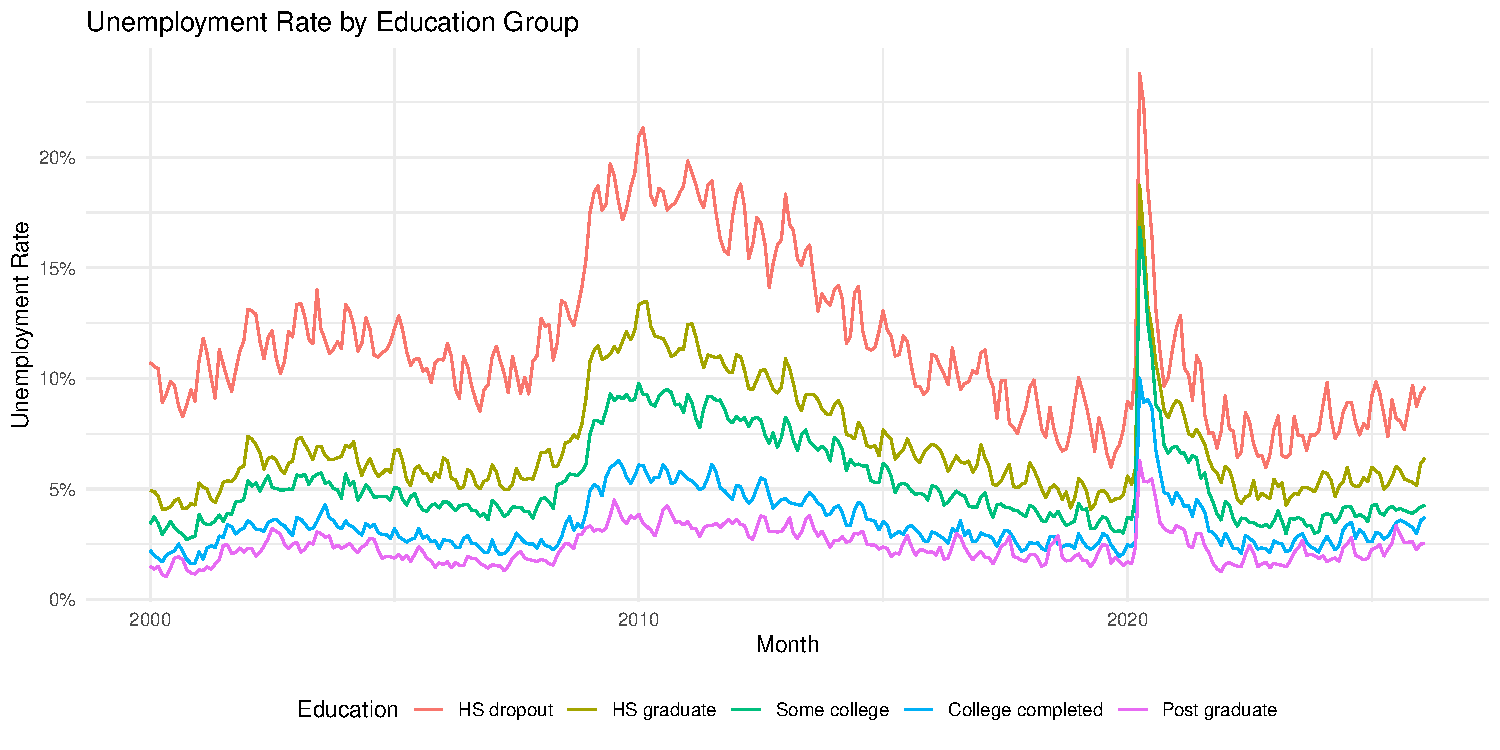
\includegraphics[width=1\textwidth]{Figures/plot_q2_1_urate_by_educ.pdf}
  \caption{Unemployment rate by education group}
  \label{fig:sample-image}
\end{figure}

The figure shows that unemployment rates are consistently lower for more educated groups.

\begin{table}[H]
\centering
\caption{Average Unemployment Rate by Education Group}
\begin{tabular}{lcc}
\hline
\textbf{Education Group} & \textbf{Avg.\ Unemployment Rate} & \textbf{Avg.\ $N$} \\ \hline
HS dropout               & 0.116                            & 6098                \\
HS graduate              & 0.070                            & 17943               \\
Some college             & 0.053                            & 17916               \\
College completed        & 0.034                            & 13607               \\
Post graduate            & 0.024                            & 7512                \\ \hline
\end{tabular}
\end{table}

\begin{table}[H]
\centering
\caption{Changes in Unemployment Rates by Education Group during Great Recession}
\begin{tabular}{lccccc}
\hline \hline
\textbf{Education Group} & $u_0$ & $u_T$ & $\Delta u$ & $N_0$ & $N_T$ \\ \hline
HS dropout               & 0.110 & 0.197 & 0.087      & 7221  & 7721  \\
HS graduate              & 0.060 & 0.111 & 0.051      & 20462 & 20556 \\
Some college             & 0.042 & 0.093 & 0.051      & 20060 & 20645 \\
College completed        & 0.023 & 0.059 & 0.036      & 13895 & 14360 \\
Post graduate            & 0.017 & 0.038 & 0.021      & 7300  & 7541  \\ \hline \hline
\end{tabular}
\end{table}

\begin{table}[ht]
\centering
\caption{Changes in Unemployment Rates During COVID-19 by Education Group}
\begin{tabular}{lccccc}
\hline \hline
\textbf{Education Group} & $u_0$ & $u_T$ & $\Delta u$ & $N_0$ & $N_T$ \\ \hline
HS dropout               & 0.086 & 0.238 & 0.152      & 4311  & 3297  \\
HS graduate              & 0.052 & 0.187 & 0.135      & 15355 & 12020 \\
Some college             & 0.036 & 0.168 & 0.132      & 16369 & 13371 \\
College completed        & 0.024 & 0.100 & 0.076      & 14467 & 12169 \\
Post graduate            & 0.016 & 0.063 & 0.047      & 8480  & 7333  \\ \hline \hline
\end{tabular}
\end{table}

\subsection*{Part 2}

\begin{figure}[H]
  \centering
  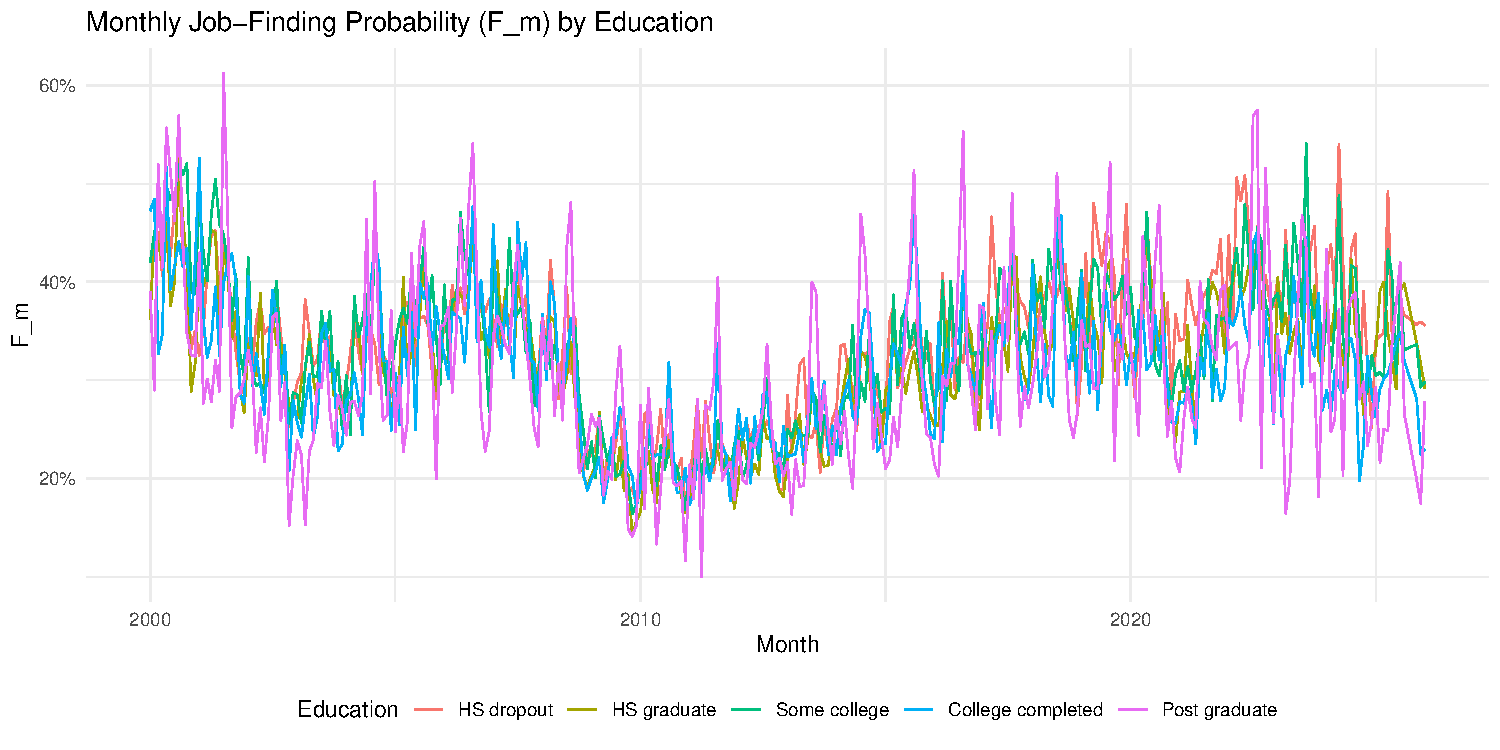
\includegraphics[width=1\textwidth]{Figures/plot_q2_2_Fm_by_educ.pdf}
  \caption{Monthly job finding probability $F_m$ by education criteria}
  \label{fig:sample-image}
\end{figure}

\begin{figure}[H]
  \centering
  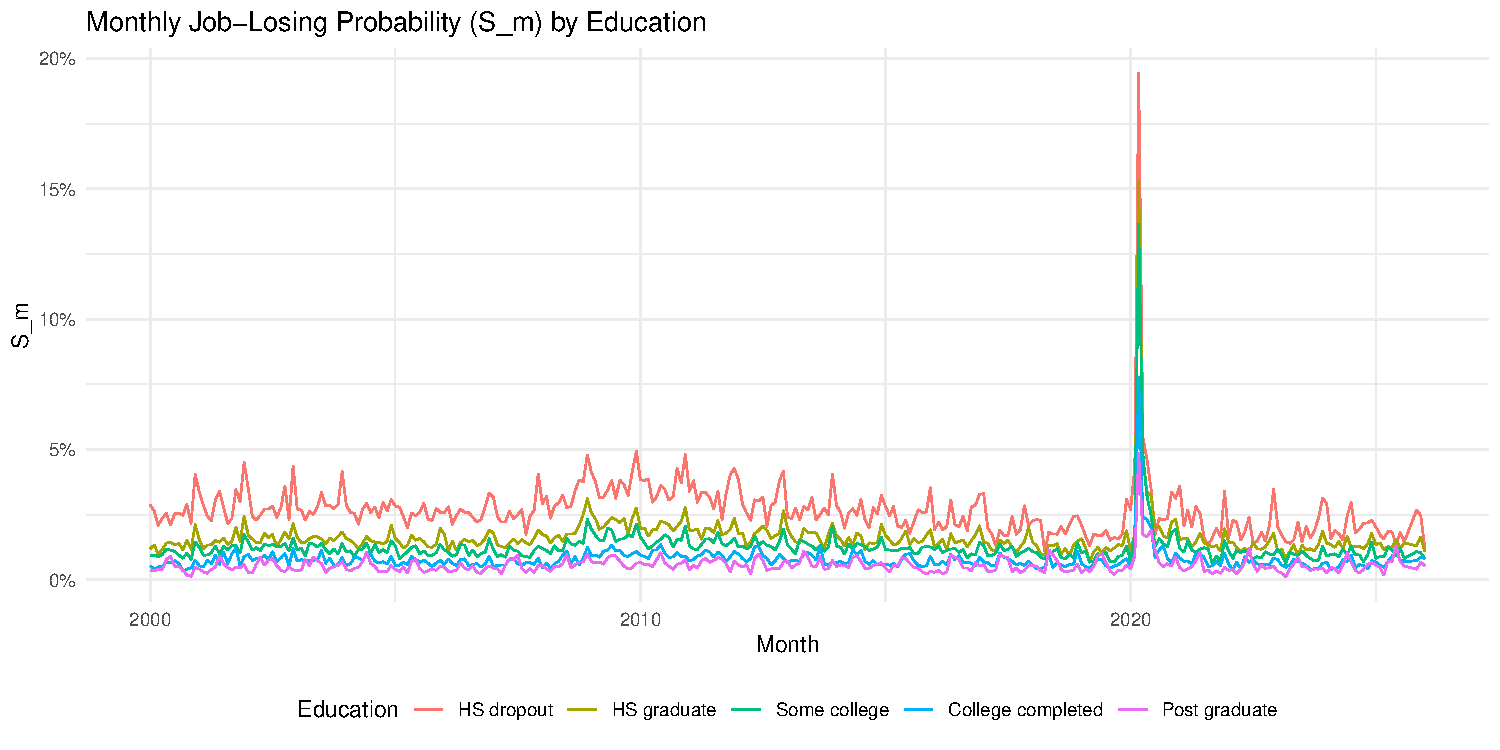
\includegraphics[width=1\textwidth]{Figures/plot_q2_2_Sm_by_educ.pdf}
  \caption{Monthly job losing probability $S_m$ by education criteria}
  \label{fig:sample-image}
\end{figure}


\subsection*{Part 3}

From equations \ref{eq:q1_fm_Fm_rel} and \ref{eq:q1_sm_Sm_rel}
\begin{align*}
    \frac{F_m}{S_m} &= \frac{f_m}{s_m} \\
    F_m + S_m &= 1-e^{-(f_m+s_m)}
\end{align*}

solving these, we get
\begin{align*}
    f_m &= -\ln(1 - F_m - S_m) \frac{F_m}{F_m + S_m}\\
    s_m &= -\ln(1 - F_m - S_m) \frac{S_m}{F_m + S_m}
\end{align*}

\begin{figure}[H]
  \centering
  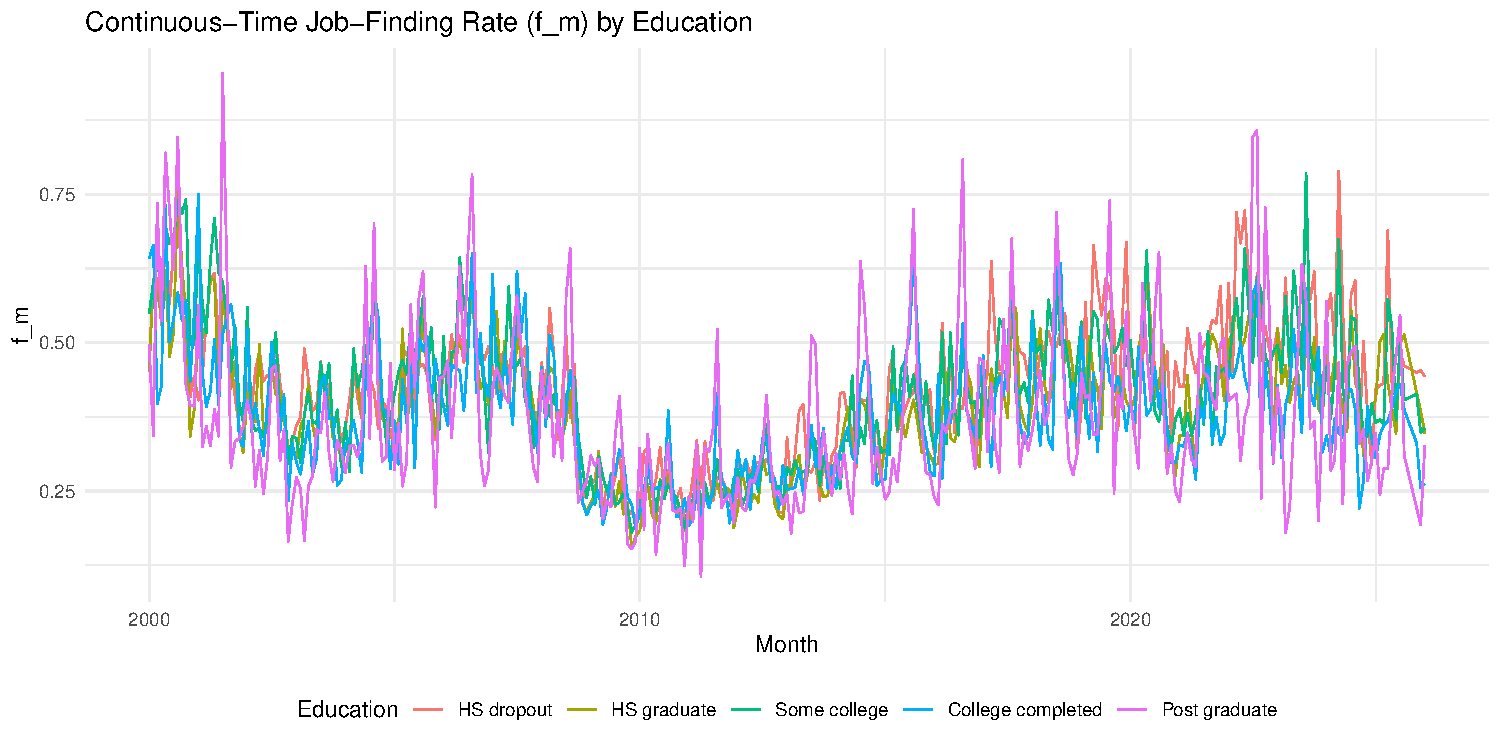
\includegraphics[width=1\textwidth]{Figures/plot_q2_3_fm_by_educ.pdf}
  \caption{Underlying job finding rates $f_m$ by education criteria}
  \label{fig:sample-image}
\end{figure}

\begin{figure}[H]
  \centering
  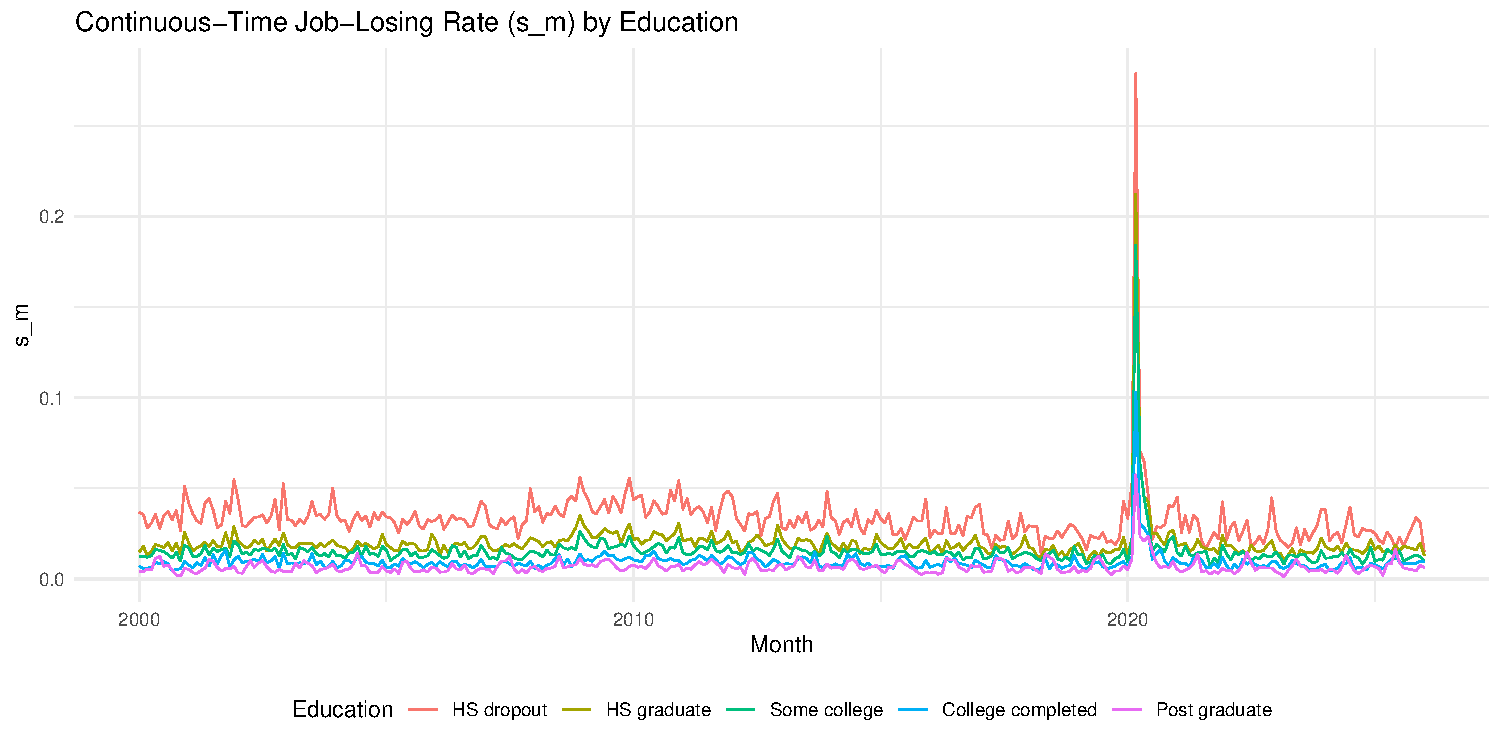
\includegraphics[width=1\textwidth]{Figures/plot_q2_3_sm_by_educ.pdf}
  \caption{Underlying job losing rates $s_m$ by education criteria}
  \label{fig:sample-image}
\end{figure}


\begin{figure}[H]
  \centering
  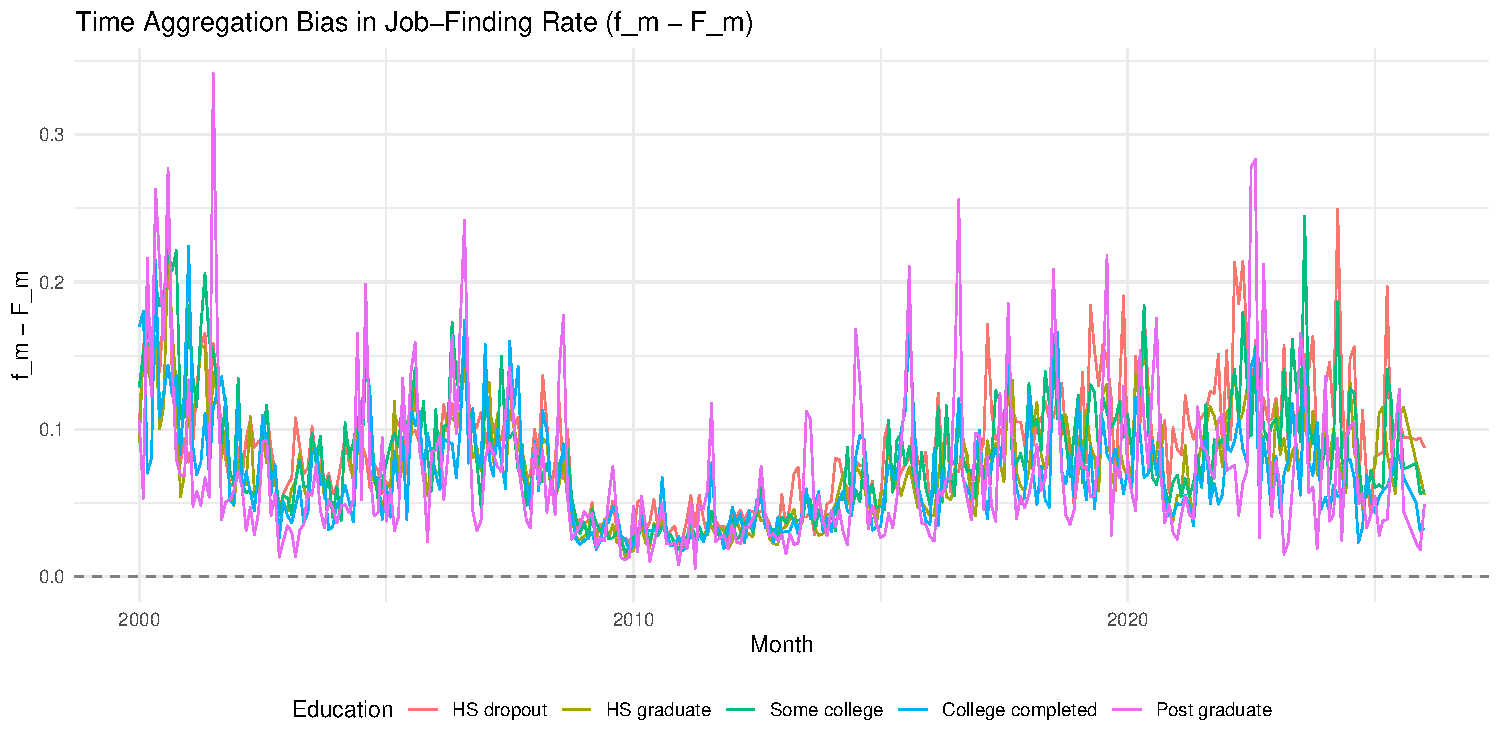
\includegraphics[width=1\textwidth]{Figures/plot_q2_3_bias_f.pdf}
  \caption{Aggregation bias in job finding rates $f_m-F_m$ by education criteria}
  \label{fig:sample-image}
\end{figure}

\begin{figure}[H]
  \centering
  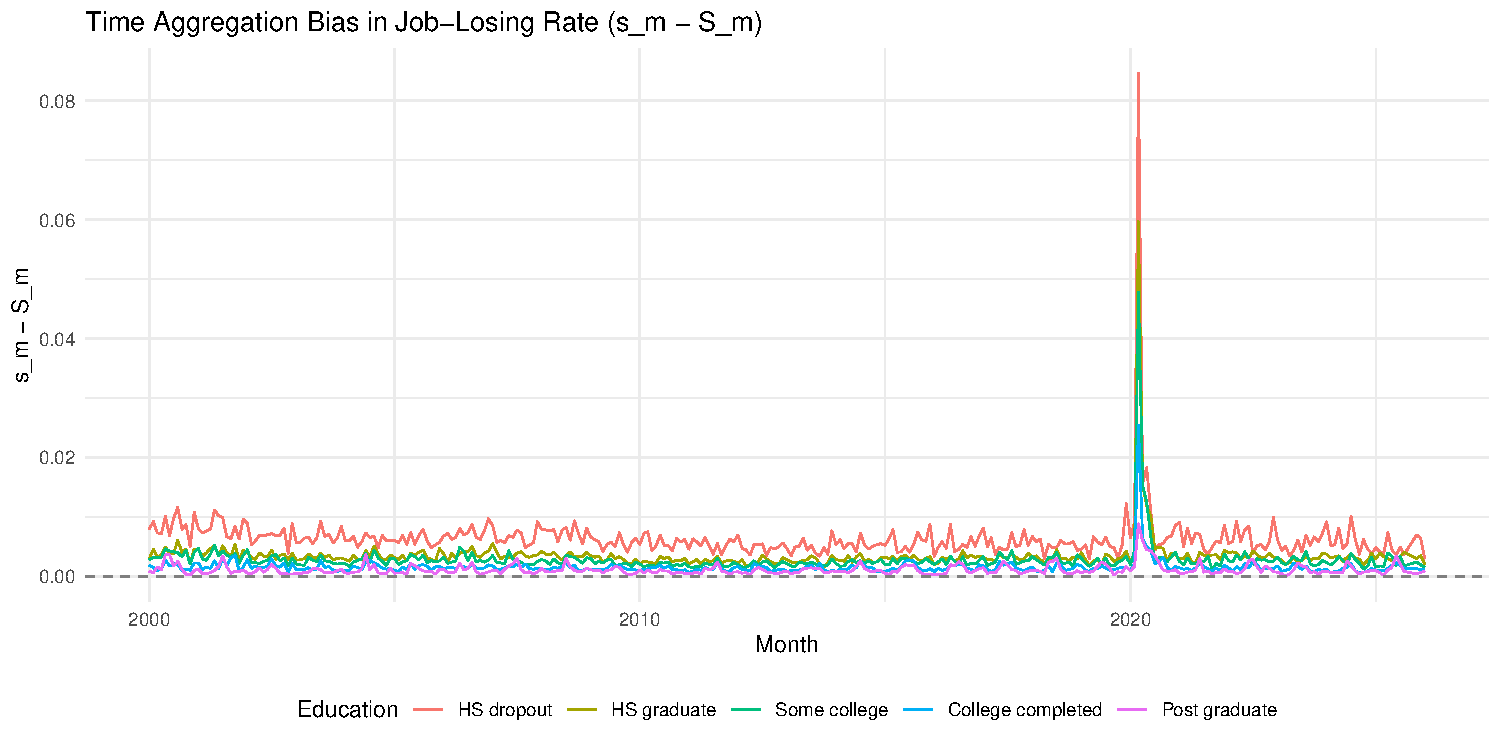
\includegraphics[width=1\textwidth]{Figures/plot_q2_3_bias_s.pdf}
  \caption{Aggregation bias in job losing rates $s_m-S_m$ by education criteria}
  \label{fig:sample-image}
\end{figure}


\subsection*{Part 4}
In month m, following lecture notes, define the quasi-equilibrium unemployment rate of education group g as 
\begin{equation}
    \hat u_m^g = \frac{S_m^g}{S_m^g + F_m^g}
\end{equation}

The share of fluctuation is given by 
\begin{align*}
    \text{flutuations due to S in month m} &= \frac{Cov_g\left[\log \frac{\hat u^g_m}{1-\hat u^g_m},
         \log s^g_m \right]}{Var_g\left[\log \frac{\hat u^g_m}{1-\hat u^g_m}\right]}\\
    \text{flutuations due to F in month m} &= \frac{Cov_g\left[\log \frac{\hat u^g_t}{1-\hat u^g_t},
         -\log f^g_m \right]}{Var_g\left[\log \frac{\hat u^g_m}{1-\hat u^g_m}\right]}
\end{align*}

where $Cov_g$ and $Var_g$ represent cross sectional covariance and variance weighted by group weights. I use $S_m, F_m$ (discrete-time probabilities) in place of $s, f$.

\subsubsection*{Levels decomposition}

\begin{figure}[H]
  \centering
  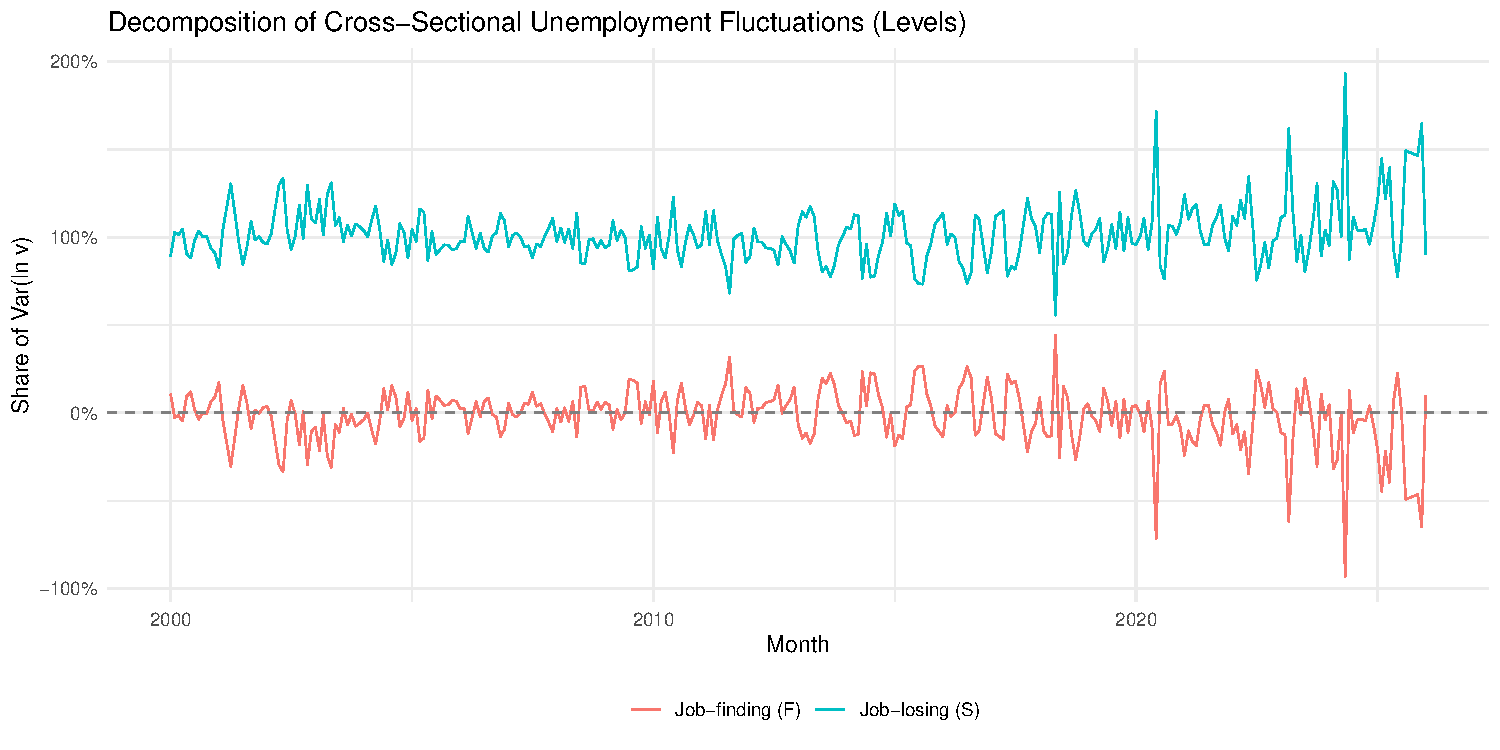
\includegraphics[width=1\textwidth]{Figures/plot_q2_4_decomp_levels.pdf}
  \caption{Decomposition of cross-sectional unemployment fluctuations (levels)}
  \label{fig:q2_4_levels}
\end{figure}

\begin{table}[H]
\centering
\caption{Mean Share of Fluctuations (Levels)}
\begin{tabular}{lc}
\hline
\textbf{Component} & \textbf{Mean Share} \\ \hline
Job-losing ($S$)   & 101.9\%               \\
Job-finding ($F$)  & -1.9\%            \\ \hline
Sum                & 100\%             \\ \hline
\end{tabular}
\end{table}

In the levels decomposition, job-losing accounts for slightly more than 100\% of the cross-sectional variance in steady-state unemployment across education groups, while job-finding has a small negative share ($-1.9\%$). This implies that across education groups, differences in $S$ more than fully explain unemployment dispersion, and differences in $F$ actually slightly compress it --- groups with higher $S$ also tend to have higher $F$, partially offsetting the effect of job-losing on unemployment.

\subsubsection*{Changes decomposition}

I also perform the same decomposition on monthly changes $\Delta \ln v$, $\Delta \ln S$, $\Delta \ln F$.

\begin{align*}
    \text{flutuations due to S in month m} &= \frac{Cov_g\left[\Delta\log \frac{\hat u^g_m}{1-\hat u^g_m},
         \Delta\log s^g_m \right]}{Var_g\left[\Delta\log \frac{\hat u^g_m}{1-\hat u^g_m}\right]}\\
    \text{flutuations due to F in month m} &= \frac{Cov_g\left[\Delta\log \frac{\hat u^g_t}{1-\hat u^g_t},
         -\Delta\log f^g_m \right]}{Var_g\left[\Delta\log \frac{\hat u^g_m}{1-\hat u^g_m}\right]}
\end{align*}


\begin{figure}[H]
  \centering
  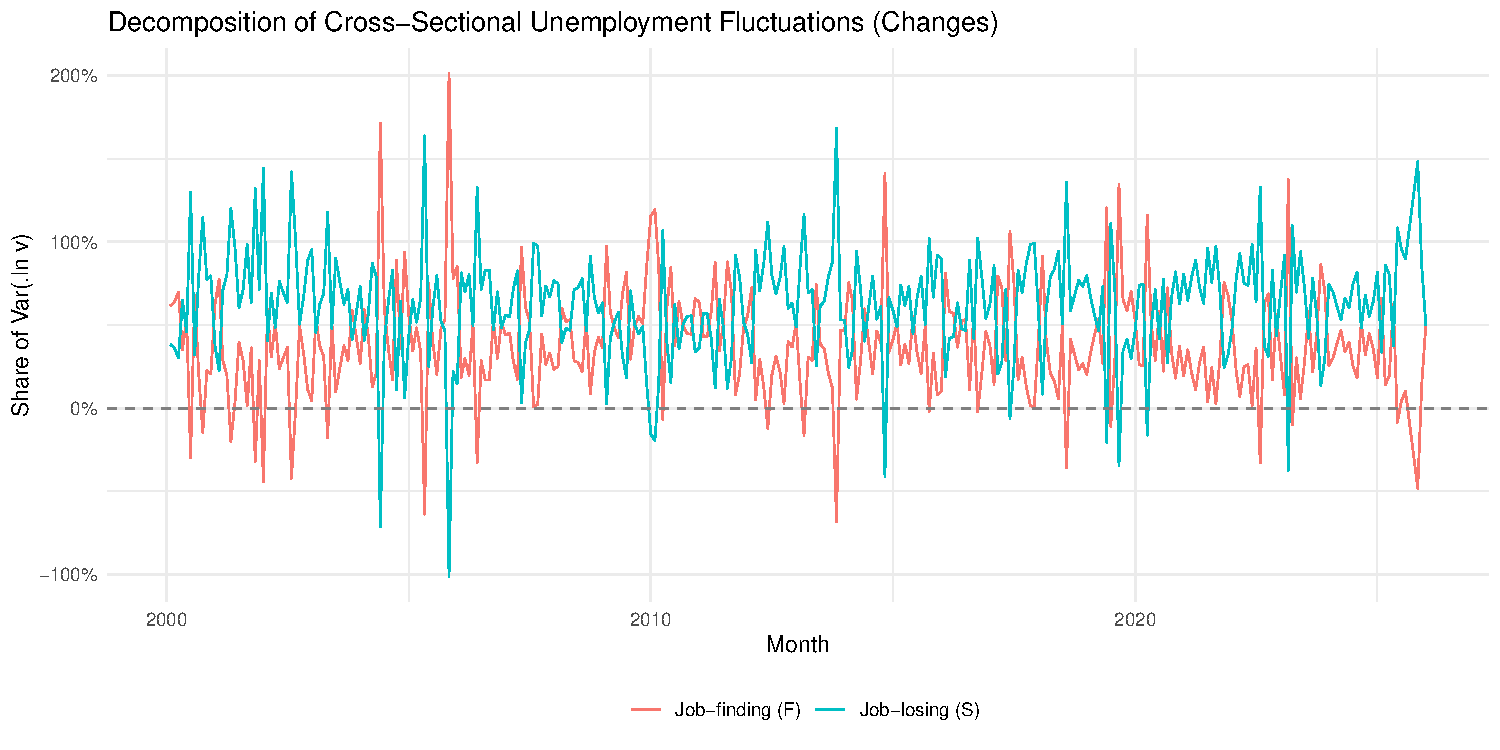
\includegraphics[width=1\textwidth]{Figures/plot_q2_4_decomp_changes.pdf}
  \caption{Decomposition of cross-sectional unemployment fluctuations (monthly changes)}
  \label{fig:q2_4_changes}
\end{figure}

\begin{table}[H]
\centering
\caption{Mean Share of Fluctuations (Monthly Changes)}
\begin{tabular}{lc}
\hline
\textbf{Component} & \textbf{Mean Share} \\ \hline
Job-losing ($S$)   & 62.0\%               \\
Job-finding ($F$)  & 38.0\%               \\ \hline
Sum                & 100 \%              \\ \hline
\end{tabular}
\end{table}

In the changes decomposition, job-losing accounts for about 62\% of the cross-sectional variance in monthly changes in steady-state unemployment, while job-finding accounts for 38\%. Both components contribute positively, indicating that month-to-month changes in the cross-sectional dispersion of unemployment are driven by both margins, with job-losing being the dominant source.

